\graphicspath{{1intro/asy/},{3cyclic/asy/}}
\thispagestyle{empty}

\section*{A Brief Review of Complex Number Notation}

The complex numbers $\C=\{x+iy:x,y\in\R\}$ are the real vector space $\R^2$ spanned by a basis $\{1,i\}$ where $i^2=-1$ is a 'number' satisfying $i^2=-1$. To multiply complex numbers, simply expand out and replace $i^2$ with $-1$: for example
\[
	(2+3i)(1-i) =2-i+3i-3i^2 =2+2i+3 =5+2i
\]

\begin{description}
	\begin{minipage}[t]{0.7\linewidth}\vspace{-10pt}
		\item[\emph{Complex conjugate}:] Given a complex number $z=x+iy\in\C$, its \emph{conjugate} $\cl z=x-iy$ is the reflection of $z$ in the real axis.
		\item[\emph{Modulus (length)}:] $r=\nm z=\sqrt{z\cl z}=\sqrt{x^2+y^2}$ is the distance of $z$ from the origin.
		\item[\emph{Argument (angle)}:] If $z\neq 0$, then $\theta=\arg z$ is the angle measured counter-clockwise from the positive real axis to the ray $\ray{0z}$.
	\end{minipage}
	\hfill
	\begin{minipage}[t]{0.28\linewidth}\vspace{-45pt}
		\flushright%
		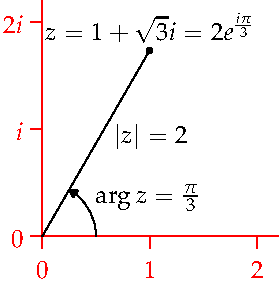
\includegraphics[scale=0.9]{cyclic-polar}%\smallbreak
		%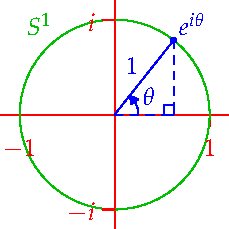
\includegraphics[scale=1]{cyclic-circle}
	\end{minipage}\par
	
	\item[\emph{Polar form}:] $z=re^{i\theta} =r\cos\theta+ir\sin\theta$. The complex exponential obeys the usual exponential laws and is $2\pi i$-periodic: for instance
	\begin{itemize}
		 \item $e^{i\theta}e^{i\psi}=e^{i(\theta+\psi)}$
		 \item $e^{i\theta}=1\iff \theta=2\pi k$ for some integer $k$
	\end{itemize}
	The modulus and argument are the usual polar co-ordinates of a point in $\R^2$. The exponential laws show that the polar form behaves nicely with respect to complex multiplication:
	\[
		\nm{zw}=\nm z\nm w\quad \text{and}\quad \arg(zw)\equiv \arg z+\arg w \pmod{2\pi}
	\]
	\begin{minipage}[t]{0.7\linewidth}\vspace{-5pt}
		\item[\emph{Euler's Formula \& the Unit Circle}:] When $r=1$ we have \emph{Euler's formula}:
		\[
			e^{i\theta}=\cos\theta+i\sin\theta
		\]
		the source of the famous identity $\displaystyle e^{i\pi}=-1$. These complex numbers comprise the \textcolor{Green}{unit circle}
		\[
			S^1 =\bigl\{z\in\C:\nm z=1\bigr\} =\bigl\{e^{i\theta}:\theta\in[0,2\pi)\bigr\}
		\]
	\end{minipage}
	\hfill
	\begin{minipage}[t]{0.28\linewidth}\vspace{-12pt}
		\flushright%
		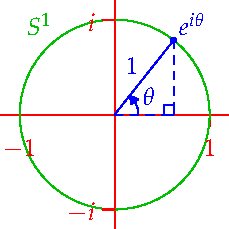
\includegraphics[scale=1]{cyclic-circle}
	\end{minipage}
	
	\item[\emph{Rotations}:] Let $\theta$ be a fixed real number. The complex function $\text{rot}_\theta(z)=e^{i\theta}z$ has the effect of \emph{rotating $z$ about the origin by $\theta$ radians.} To see why, write $z=re^{i\psi}$ in polar form and observe that
	\[
		\text{rot}_\theta(z)= e^{i\theta}re^{i\psi}=re^{i(\theta+\psi)}
	\]
	has the \emph{same modulus} $r$, but has had \emph{$\theta$ radians added to its modulus.} For this reason, the unit circle $S^1$ can be thought of as the set of \emph{rotations around the origin.} 
\end{description}

	